\section{Built a mechanism that reduces the size of queries}\label{section:applied-methods:query-reduction}

After implementing the shared caching layer, the next step was to improve the performance of the micro-frontends by optimizing the use of the cache. The size of the network requests can be reduced by removing parts of a query that are already inside the cache. The theory behind removing fields from the query was already explained in Section \ref{subsection:background:graphql:query-reduction}. The Apollo Client does not provide such a functionality out of the box, but many users request the feature in Apollo's Github Repository. Section \ref{subsubsection:background:graphql:apollo-server-client:in-memory-cache-working} explains how the \texttt{InMemoryCache} of Apollo Client works in more detail. Briefly summarized the caching works with the name and the parameters of a GraphQL query. For example, if a query is executed against the GraphQL \ac{API}, the results of the query are cached. If the same query with the same fields is executed again with the same parameters, the results are fetched from the Apollo Client cache. If the query fetches an additional field, not inside the cache, the complete query is sent to the GraphQL \ac{API}. Only if the queried fields are identical the cache data is used. Consequently, identical queries that fetch different fields are always fetched from the server.

\bigskip

\noindent Consider Listing \ref{code:applied-methods:compare-allusers-user-query}, where the left query fetches all users, and the query on the right fetches a user by its id. Both queries fetch the same data type and the same fields, but they are fundamentally different queries. They have different names and different parameters. Both queries are sent to the GraphQL \ac{API}. The query on the right could be omitted if the user with the given id is fetched from the cache. If the left query is executed before the query on the right, the data to resolve the query on the right could be taken entirely from the cache.

\ifshowListings
\begin{listing}[H]
\begin{minted}{typescript}
query allUsers {                        query user(id: ID!) {
  allUsers {                              user(id: id) {
    id                                      id
    username                                username
    email                                   email
    firstName                               firstName
    secondName                              secondName
  }                                       }
}                                      }
\end{minted}
\caption{Compare the fields between the \texttt{allUsers} and \texttt{User} query.}\label{code:applied-methods:compare-allusers-user-query}
\end{listing}
\fi

\noindent Apollo Client offers a solution to tackle this problem. The application might have a detail view and a list view that query the same data as in Listing \ref{code:applied-methods:compare-allusers-user-query}. The user query data might already be in the cache, but the Apollo Client does not know that. Therefore, the cache lookup can be configured so the Apollo Client knows where to look for the data. A basic understanding of type policies is needed to understand the cache redirection, described in more detail in Section \ref{subsubsection:background:graphql:apollo-server-client:type-policies}.

\bigskip

\noindent A field policy \texttt{read} function must be written for the user query to inform the Apollo Client where to look for the cached \texttt{User} object. Like the \texttt{firstName} being a \texttt{User} type field, the user query is a field of the root query. This hierarchy resembles the structure of the GraphQL Schema, where the queries have to be defined inside the \texttt{Query} type. Listing \ref{code:applied-methods:query-reduction:graphql-schema} shows an excerpt from the GraphQL schema. All queries that a client can execute are listed inside the \texttt{Query} type.

\ifshowListings
\begin{listing}[H]
\begin{minted}{typescript}
type Query {
  user(id: ID!): User
  allUsers(page: Int, perPage: Int): [User]
  ...
}

type User {
  id: ID!
  firstName: String!
  secondName: String!
  ...
}
\end{minted}
\caption{An excerpt of the prototypes GraphQL schema.}\label{code:applied-methods:query-reduction:graphql-schema}
\end{listing}
\fi


\noindent Listing \ref{code:applied-methods:query-reduction:user-cache-redirect} shows the \texttt{read} field policy for the \texttt{User}. Like in the GraphQL schema from Listing \ref{code:applied-methods:query-reduction:graphql-schema}, the user query is a field of the root query. Therefore, the read function is executed every time the client runs the user query. The \texttt{toReference} function is used to cache a reference for a \texttt{User} type. The reference is generated based on its \texttt{\_\_typename} and \texttt{id}, as explained in Section \ref{subsubsection:background:graphql:apollo-server-client:data-normalization}. Apollo Client uses the result of \texttt{toReference} to look up the object in its cache and return it if it is present. The query is sent to the GraphQL \ac{API} if the object is not in the cache.

\ifshowListings
\begin{listing}[H]
\begin{minted}{typescript}
new ApolloClient({
  cache: new InMemoryCache({ typePolicies: { Query: { fields: {
    User: {
      read(_, { args, toReference }): {
        return toReference({ __typename: 'User', id: args.id });
      }
    }
  }}}})
});
\end{minted}
\caption{A cache-redirect for the User-type.}\label{code:applied-methods:query-reduction:user-cache-redirect}
\end{listing}
\fi

\noindent Using cache redirects to reduce the amount of network requests works, but all of the query's requested fields must be already present in the cache. If the user query fetches any field that the \texttt{allUsers} query did not, Apollo Client considers the cache hit incomplete, and the query is executed over the network. That a detail view and a list view are perfectly identical is very rare in applications. Therefore, this approach cannot effectively reduce the size of network requests. Moreover, the approach is very verbose because a redirect has to be written for every data type. The approach does not scale; the same type-policies must be written and registered for every micro-frontend.

\bigskip

\noindent The open-source project \textbf{apollo-augmented-hooks}\footnote{\url{https://github.com/appmotion/apollo-augmented-hooks}} on GitHub provides drop-in replacements for Apollo's GraphQL query methods. It provides the functionality to remove fields from a query already in the cache. However, the big problem is that the project was developed specifically for React's Apollo Client. The dependencies were outdated, and the latest release of the library was in 2021. The library's functionality could only be tested with an old Apollo Client and React version. The dependency offered the functionality to remove fields in the cache from a previous GraphQL query. The \textbf{apollo-augmented-hooks} dependency was forked to use the functionality of the library inside the prototypical micro-frontend architecture. The first step was to update the dependencies to make it work with the latest version of Apollo Client. The problem with the old implementation is that it just supports React's Apollo Client with its hooks. The core functionality of the library was extracted, and an adapter for React and Angular was written utilizing the functionality. The functions have the same \ac{API} as Apollo Client's original methods, so migration to the new functions is straightforward. The library's functionality was rewritten with \ac{TS}, adding additional features that utilize the cache even more. The implementation is detailed further in Section \ref{subsection:applied-methods:query-reduction:how-does-the-library-work}.

\ifshowAppliedMethodsTestingQueryReduction
  \subsection{Implementing a query reduction testing layer}\label{subsection:applied-methods:query-reduction:testing-query-reduction}

The following abstraction, seen in Listing \ref{code:applied-methods:query-reduction:graphql-client} for the GraphQL client, was created to compare the Apollo Client's default behavior with the improved behavior of reducing queries.The \texttt{watchQuery} and \texttt{mutate} functions have the same \ac{API} as Apollo Client's original query and mutate functions. Two implementations (\texttt{ReduceGraphQLClientImpl}, \texttt{GraphQLClientImpl}) were created for the base class \texttt{GraphQLClient}. The \texttt{ReduceGraphQLClientImpl} uses query reduction, while \texttt{GraphQLClientImpl} utilizes the original Apollo Client functions. A switch is used to determine which implementation is created at runtime.

\ifshowListings
\begin{listing}[H]
\begin{minted}{typescript}
abstract class GraphQLClient {
  abstract watchQuery<TData, TVariables>(
    options: WatchQueryOptions<TData, TVariables>
  ): Observable<QueryResult<TData>>;

  abstract mutate<TData, TVariables>(
    options: MutationOptions<TData, TVariables>
  ): Observable<MutationResult<TData>>;
}
\end{minted}
\caption{The abstract base class for the GraphQL client.}\label{code:applied-methods:query-reduction:graphql-client}
\end{listing}
\fi

\noindent The switch is implemented as a \ac{DI} token, which can be specified in the applications. The \texttt{REDUCE\_QUERY\_OPTIONS} injection token determines whether the query reduction should be used. The usage of the token is shown in the Listing \ref{code:applied-methods:query-reduction:switch-between-apollo-client-and-query-reduction}. The switch decides whether the \texttt{ReduceGraphQLClientImpl} or \texttt{GraphQLClientImpl} is created. The \texttt{ReduceGraphQLClientImpl} is created when the \texttt{reduceQueries} property is set to \texttt{true}. The provider is specified inside the core module of the application to create the provider globally.

\ifshowListings
\begin{listing}[H]
\begin{minted}{typescript}
const REDUCE_QUERY_OPTIONS = 
  new InjectionToken<ReduceQueryOptions>('reduce-query-options');

@NgModule({
  providers: [{
    provide: REDUCE_QUERY_OPTIONS,
    useValue: { reduceQueries: true },
  }]
})
class ContactCoreModule {}
\end{minted}
\caption{Specify whether queries should be reduced.}\label{code:applied-methods:query-reduction:switch-between-apollo-client-and-query-reduction}
\end{listing}
\fi


\fi

\subsection{Query reduction mechanism}\label{subsection:applied-methods:query-reduction:how-does-the-library-work}

This section briefly describes how the query reduction functionality removes fields from the query using the \texttt{InMemoryCache}. Apollo Client allows specifying multiple configuration options when fetching a query from a GraphQL \ac{API}. Three important options are \texttt{variables}, \texttt{query}, and \texttt{fetchPolicy}. The \texttt{query} specifies the GraphQL query, and the \texttt{variables} are the variables for the query. The fetch policy lets the client specify how data is stored and retrieved from the cache. The typical structure of a GraphQL query inside the micro-frontend architecture is shown in Listing \ref{code:applied-methods:query-reduction:executing-graphql-query}. The query fetches the user's details with the given \texttt{id}. The default fetch policy of a query is \texttt{cache-first}.

\ifshowListings
\begin{listing}[H]
\begin{minted}{typescript}
this.graphQLClient.watchQuery({
  variables: { id: `36bad921-8fcf-4f33-9f29-0d3cd70205c8` },
  query: USER_BY_ID_QUERY,
  fetchPolicy: 'cache-first',
});
\end{minted}
\caption{Defining and running a GraphQL query with Apollo Client.}\label{code:applied-methods:query-reduction:executing-graphql-query}
\end{listing}
\fi

\noindent The Apollo Client offers several fetch policies that customize how the client retrieves data from the cache. The available fetch policies are: \cite{misc:-:applied-methods:query-reduction:apollo-client:queries}

\begin{itemize}
  \item \textbf{cache-first (default)}: This fetch policy instructs the Apollo Client first to check the local cache for the query result. If the data is present in the cache, it is returned immediately. Otherwise, Apollo Client will execute the query and fetch the result from the server, which will then be cached.
  \item \textbf{cache-and-network}: This fetch policy combines the cache-first and network-only policies. Apollo Client first checks the cache for the query result and returns it immediately if it is present. Then, a network request is made to fetch the most up-to-date data, which is then used to update the cache. This fetch policy is a good option for displaying data that gets updated frequently.
  \item \textbf{cache-only}: This fetch policy tells Apollo Client only to check the cache for the query result. If the result is present in the cache, it is returned immediately.
  \item \textbf{network-only}: This fetch policy instructs Apollo to skip the cache entirely and always fetch the query result from the server.
  \item \textbf{no-cache}: This fetch policy skips the cache entirely and always fetches the query result from the server. Unlike network-only, the result is not cached.
\end{itemize}

\noindent The first step of the function is whether the fetch policy allows the query to be reduced. Suppose the query is executed with one of the following cache policies: \texttt{cache-only}, \texttt{network-only}, and \texttt{no-cache}; reducing the query is counterproductive. With \texttt{network-only}, the latest data should be fetched from the GraphQL \ac{API}. The \texttt{cache-only} policy only targets the cache; therefore, no reduction is necessary. The no-cache policy bypasses the cache and requests data from the GraphQL \ac{API}. Another feature of Apollo Client is polling. Polling in Apollo Client is a technique used to fetch a query's data at a specified interval periodically, and it allows a near-real-time synchronization with the server. To enable polling for a query, pass a \texttt{pollInterval} (ms) configuration option to the \texttt{watchQuery} method. Removing fields from a query that uses polling does not make sense either because real-time data should be rendered. The following sections describe the steps needed to reduce the query.

\subsubsection{Identify key fields of every GraphQL type}

The first step is identifying the key fields of the types inside the schema. The contents of the \texttt{InMemoryCache} can be extracted using the \texttt{cache.extract()} function. This function returns an object with all the contents of the cache. The key fields can be read from the configuration of the cache. The implementation returns an object where the type name is the key and the key fields are the value. The \texttt{InMemoryCache} uses key fields to generate cache \acp{ID} for individual types. By default, the \texttt{id} or \texttt{\_id} of the type is used as the unique \ac{ID}. To make the query reduction work, fetching the key field of the type is necessary. A type policy must be defined for the type that should be customized. The definition of a custom key field for a type is shown in Listing \ref{code:applied-methods:query-reduction:defining-a-custom-key-field}. The \texttt{name} is used instead of the \texttt{id} to generate the cache \ac{ID} of a \texttt{Salutation}. The GraphQL API does not provide an \ac{ID} field; the name is unique. \cite{misc:-:background:graphql:apollo-client-cache-configuration}

\ifshowListings
\begin{listing}[H]
\begin{minted}{typescript}
new InMemoryCache({
  typePolicies: {
    Salutation: { keyFields: ['name'] }
  }
});
\end{minted}
\caption{Defining a custom key field for the Salutation type.}\label{code:applied-methods:query-reduction:defining-a-custom-key-field}
\end{listing}
\fi

\noindent The reduction process cannot remove the key fields of a type because they are the unique identifier of the data entry inside the cache. Apollo Client needs this \ac{ID} to determine if an entity with the same \ac{ID} already exists in the cache. If it does, the Apollo Client will try to merge the incoming data with the existing data; otherwise, it will create a new cache entry.

\subsubsection{Check the data of the cache}

After storing the key fields for every type, the selected fields of the query are iterated. For example, listing \ref{code:applied-methods:query-reduction:selection-set-query} shows a GraphQL query that fetches all salutations and all titles. The selection set of this combined query is an array containing \texttt{allSalutations} and \texttt{allTitles}.

\ifshowListings
\begin{listing}[H]
\begin{minted}{typescript}
query {
  allSalutations {
    id
    name
  }
  allTitles {
    id
    name
  }
}
\end{minted}
\caption{A combined GraphQL query that fetches two datasets.}\label{code:applied-methods:query-reduction:selection-set-query}
\end{listing}
\fi

\noindent The names of the queries can be used to check whether the query was executed before and was cached. Therefore, the identifier of the query inside the cache must be determined. The query's name inside the cache is concatenated with the query variables by default. The arguments are converted to a string that has the following structure \texttt{(\{variableName:value,variableName:value,\dots\})}. If the query is executed with different arguments, it has a separate entry inside the cache. The arguments of a query are converted to key-value pairs. For example, the following query shown in listing \ref{code:applied-methods:query-reduction:storing-a-query-with-arguments} fetches a contact by its \ac{ID} and reads the \texttt{id} from the contact.

\ifshowListings
\begin{listing}[H]
\begin{minted}{typescript}
query {
  contact(id: "36bad921-8fcf-4f33-9f29-0d3cd70205c8") {
    id
  }
}
\end{minted}
\caption{Fetching a contact by id.}\label{code:applied-methods:query-reduction:storing-a-query-with-arguments}
\end{listing}
\fi

\noindent After the GraphQL query was fetched from the GraphQL \ac{API}, the contents of the \texttt{InMemoryCache} are shown in listing \ref{code:applied-methods:query-reduction:cache-representation-of-query-with-arguments}. The cache entry is the name of the query with the parameters of the query joined together. If the same query is executed with different arguments, there would be a separate cache entry inside the \texttt{ROOT\_QUERY} object.

\ifshowListings
\begin{listing}[H]
\begin{minted}{typescript}
{
  ROOT_QUERY {
    'contact({"id":"36bad921-8fcf-4f33-9f29-0d3cd70205c8"})': {
      __ref: 'Contact:36bad921-8fcf-4f33-9f29-0d3cd70205c8'
    }
  },
  'Contact:36bad921-8fcf-4f33-9f29-0d3cd70205c8': {
    __typename: 'Contact',
    id: '36bad921-8fcf-4f33-9f29-0d3cd70205c8'
  }
}
\end{minted}
\caption{The contents of the cache after fetching the query from listing \ref{code:applied-methods:query-reduction:storing-a-query-with-arguments}.}\label{code:applied-methods:query-reduction:cache-representation-of-query-with-arguments}
\end{listing}
\fi

\noindent To check whether the query was executed before, the query's name to reduce and its arguments must be put into the form of how the cache stores them. If no arguments are present, the name of the query is stored as the name inside the cache, without the round brackets. The forked library did not account for queries that do not have arguments, and the implementation did not check whether any arguments were set. It stringified the empty arguments object, which resulted in the library checking the \texttt{ROOT\_QUERY} with the argument value \enquote{(\{\})} instead of only the name directly. This leads to a cache miss and the query can't be reduced, although the query would have been cached. The adaption to the library is shown in Listing \ref{code:applied-methods:query-reduction:determine-the-field-name}, where the name of the query is returned directly if no arguments are present.

\bigskip

\noindent Another difference from the original implementation was that key args of the type were not considered. Key arguments are used to configure field policies for caching, specifying which arguments should be used as part of the cache key for a particular field. For example, if a \texttt{User} is queried with the \texttt{id} 1 and 2, the Apollo Client stores two entries for both. By default, the cache stores separate entries for each unique combination of field arguments. Each storage key includes the corresponding argument values. If a field has no arguments, its storage key is just its name. The cache must determine whether it can merge the values returned for different argument combinations without invalidating data. The cache should not merge the querying results for Users with ids 1 and 2. A key argument is an argument for a GraphQL field that's included in cache storage keys for that field. \cite{misc:-:applied-methods:query-reduction:key-args}

\bigskip

\noindent The original implementation has not taken into account that the client might have set individual \texttt{keyArgs} for a query. Therefore it considers all given arguments as \texttt{keyArgs}. Like the key fields, the key args for every type can be read from the cache configuration. Only if a given argument of the query is a key argument, the GraphQL argument is considered for the cache key. Unnecessary arguments are filtered out, and the filtered arguments are then used to determine the field name of the query. A part of the logic to determine the field name of the query inside the cache is shown inside Listing \ref{code:applied-methods:query-reduction:determine-the-field-name}.

\ifshowListings
\begin{listing}[H]
\begin{minted}{typescript}
if (Object.keys(queryArgs).length === 0)
  return fieldSelection.name.value;

const filteredQueryArgs = Object.keys(queryArgs)
  .filter((key) => key in keyArgs)
  .reduce((obj, key) => {
    return Object.assign(obj, {
      [key]: queryArgs[key],
    });
  }, {});

const stringifiedArgs = stringify(filteredQueryArgs);
return `${fieldSelection.name.value}(${stringifiedArgs})`;
\end{minted}
\caption{Finding the name of the query inside the \texttt{InMemoryCache}.}\label{code:applied-methods:query-reduction:determine-the-field-name}
\end{listing}
\fi

\subsubsection{Accessing the cached data}

\noindent After the field name is determined, the \texttt{ROOT\_QUERY} of the cache object is checked, whether it contains the query's name. Listing \ref{code:applied-methods:query-reduction:getting-cache-content} shows how the contents of the cache are accessed programmatically. If the result of the access is undefined, the query's results were not cached before, and the query has to be executed entirely against the cache; otherwise, a reference to the cached data is returned. This cache reference is used to locate and read the actual data from the cache and use the existing fields to reduce the fields inside the query. All fields inside the query and the cache reference can be removed from the query, except key fields. If the query fetches a list, all cache objects must have the fields from the query. Otherwise, the fields cannot be removed from the query.

\ifshowListings
\begin{listing}[H]
\begin{minted}{typescript}
const cacheObjectsOrRefs = cacheContents['ROOT_QUERY']?.[fieldName];
\end{minted}
\caption{Accessing the cached data for a query.}\label{code:applied-methods:query-reduction:getting-cache-content}
\end{listing}
\fi

\noindent Another feature that differs from the original implementation is that additional cache references can be passed to the query by the client. These references are used to look up data inside the cache when the initial check for the query name returns undefined. The reference to the object is then used to look up the fields that can be reduced. As explained in Section \ref{section:applied-methods:query-reduction}, caching works on the query level, and the data for a query could already be fetched with another query. The client knows that some parts of the desired data are already in the cache and can pass a reference to the query. Listing \ref{code:applied-methods:query-reduction:passing-an-additional-cache-ref} shows how additional cache references are passed to the query. The function \texttt{cache.identify} is used to generate a valid cache reference for the user based on its \texttt{id}. The process respects and considers the settings of the cache and generates a valid reference based on the key fields. However, this feature works only in collaboration with cache redirects. To make the \texttt{InMemoryCache} aware that the user's data can be found somewhere else, a cache redirect, like in listing \ref{code:applied-methods:query-reduction:user-cache-redirect}, has to be defined.

\ifshowListings
\begin{listing}[H]
\begin{minted}{typescript}
const userRef = this.cache.identify({ id, 'User' });

this.graphQLClient.watchQuery({
  variables: { id },
  query: USER_DETAIL_BY_ID_QUERY,
  additionalCacheRefs: userRef ? [{ __ref: userRef }] : []
})
\end{minted}
\caption{Provide the GraphQL query reduction with additional information about the cache.}\label{code:applied-methods:query-reduction:passing-an-additional-cache-ref}
\end{listing}
\fi

\subsubsection{Querying the data}

\noindent After removing unnecessary fields from the query, the reduced query is executed against the GraphQL \ac{API}. The original query is executed just against the cache with the fetch-policy \texttt{cache-only}. The results of both operations are merged to fetch all of the fields that the original query selects, a part of this logic is seen in Listing \ref{code:applied-methods:query-reduction:combining-the-results}. If a query cannot be reduced because no existing data is available in the cache to reduce it, the original query is executed against the GraphQL \ac{API}.

\ifshowListings
\begin{listing}[H]
\begin{minted}{typescript}
this.graphqlClient
  .watchQuery({
    ...options,
    query: reducedQuery || query,
    variables,
    fetchPolicy: reducedQuery ? options.fetchPolicy : 'cache-first',
  })
  .valueChanges.pipe(
    switchMap((data) =>
      this.graphQLClient.query(
        { query, variables, fetchPolicy: 'cache-only' }
      )
      .map((completeData) => ({ ...data, data: completeData.data }))
    )
  )
\end{minted}
\caption{Combining the results of the reduced- and original-query.}\label{code:applied-methods:query-reduction:combining-the-results}
\end{listing}
\fi


\subsection{Example query reduction}\label{subsection:background:graphql:example-reduction}

This section contains an example of how the query reduction is made with the help of \textbf{apollo-augmented-hooks} functionality. The client first navigates to a tabular view of all users. This page executes the GraphQL query shown in Listing \ref{code:applied-methods:query-all-users}. After the query is fetched from the GraphQL \ac{API}, the fields in the query are cached inside Apollo's \texttt{InMemoryCache}.

\ifshowListings
\begin{listing}[H]
\begin{minted}{typescript}
query allUsers {
  allUsers {
    id
    username
    email
    password
    firstName
    secondName
    Title { id }
    Salutation { id }
  }
}
\end{minted}
\caption{A GraphQL query to fetch all users.}\label{code:applied-methods:query-all-users}
\end{listing}
\fi

\noindent Afterwards, the client navigates to the detail view of a specific user. The left GraphQL query shown in Figure \ref{fig:applied-methods:comparison-user-reduced-user} is the original query that would normally be fetched from the GraphQL \ac{API} without reducing the query. However, with the help of reducing the query with already existing data, the query on the right is sent to the GraphQL \ac{API}. Exactly the fields which were queried with the GraphQL query shown in Listing \ref{code:applied-methods:query-all-users} are removed. Therefore, 8 of the 16 fields from the query were removed, which reduces the number of queried fields by 50\%. The next chapter goes into more detail, about the impact of reducing queries by utilizing the \texttt{InMemoryCache}.

\ifshowImages
  \begin{figure}[H]
  \centering
  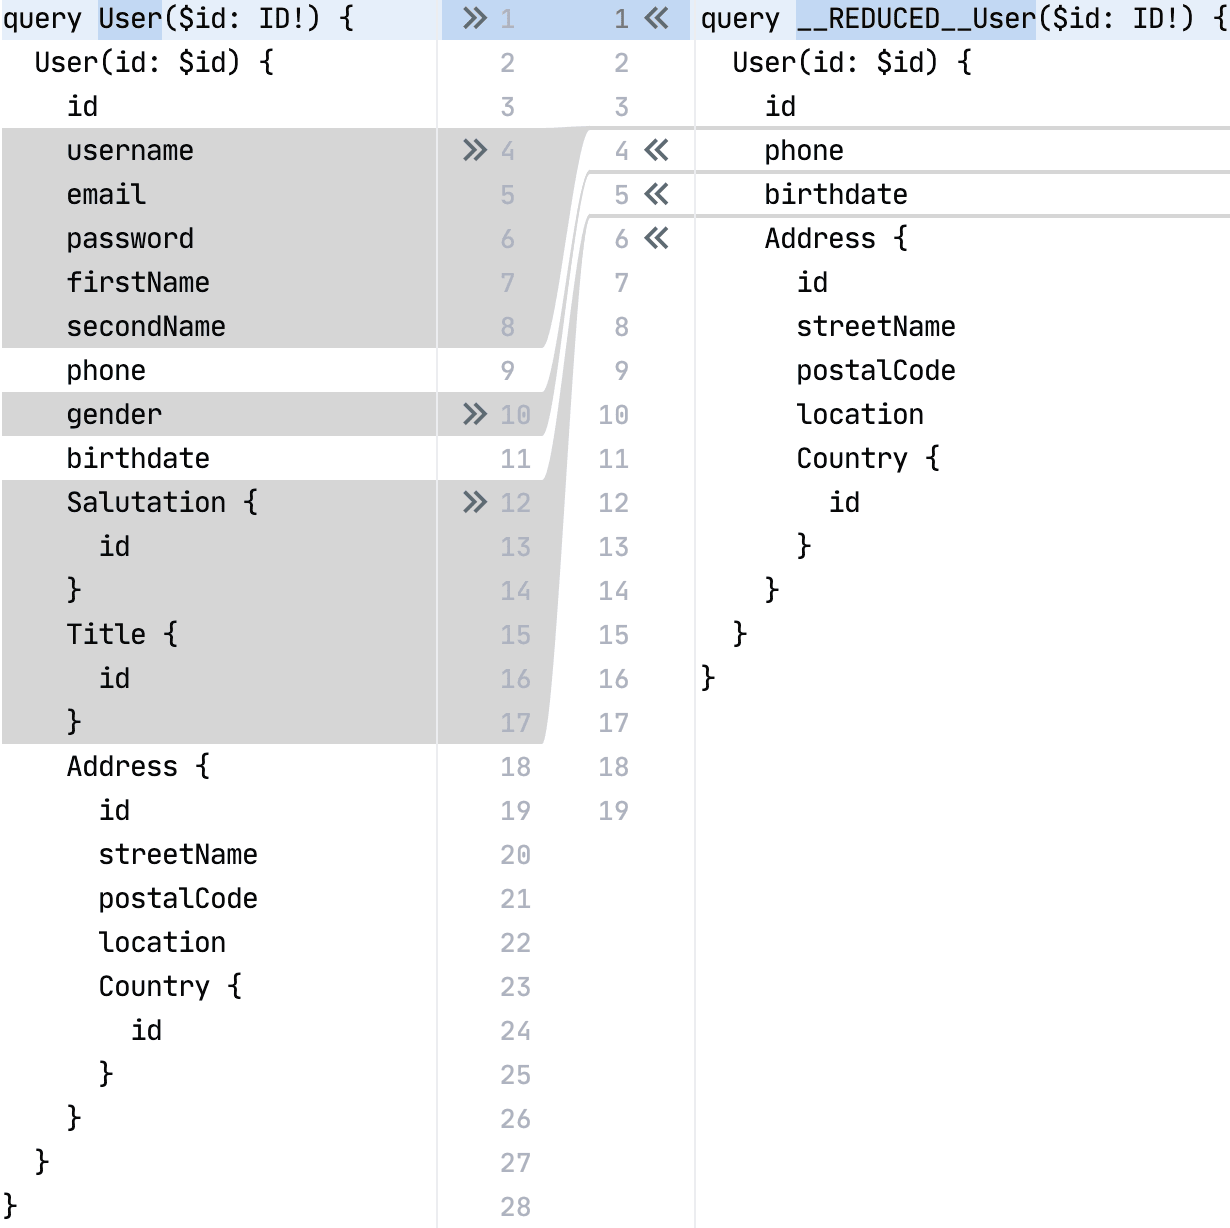
\includegraphics[width=0.65\linewidth]{images/reduction-graphql-examples/compare-user-reduced-user.png}
  \caption{A comparison of the original user- and reduced user-query.}\label{fig:applied-methods:comparison-user-reduced-user}
  \end{figure}
\fi

